% LaTeX Article Template
\documentclass{article}
\usepackage{amssymb, amsmath, amsfonts, amsthm, latexsym}
\usepackage{graphicx}
\newcommand{\C}{\mathbb {C}}
\newcommand\tab[1][1cm]{\hspace*{#1}}
\newcommand\smalltab[1][0.3cm]{\hspace*{#1}}

\begin{document}

\begin{center}
\textbf{CSCI 362 Deliverable 1: SugarLabs}
\end{center}


\begin{center}

{The Chocolate L'Eclercs}\\
\vspace{0.2cm}
{Alex Skiff, Blaine Billings, Carson Barber}\\
{Chase Myers, Justin Willis}\\
\vspace{0.2cm}

\end{center}



\begin{abstract}
\end{abstract}

\section{Chapter 1: Installation}
\subsection{Clone and Build}
In order to obtain a local instance of the project, we accessed the \textbf{sugar} repository made by the \textbf{SugarLabs} project team on GitHub\footnote{https://github.com/sugarlabs/sugar}. Using the command 
\begin{center}
\textbf{git clone sugarlabs/sugar},
\end{center}
we were, then, able to clone the project to our local machines.

From there, we utilized a document written by the SugarLabs development team included in the root directory, \textbf{README.md}, to guide the process of building the project on the operating system we chose to employ, Ubuntu 16.04. This consisted of running the following commands:
\begin{itemize}
\itemsep-0.5em
\item[] sudo apt-get install sugar-* -y
\item[] aclocal
\item[] sudo apt-get install intltool libglib2.0-dev gtk+-3.0 -y
\item[] ./autogen.sh
\item[] make
\item[] make install
\end{itemize}
\subsection{Existing Tests}
SugarLabs provided multiple testing files for ease of use. After finding the files from the root directory, we searched Python's documentation for \textbf{unittest}, the imported package used for running the test cases. Through the use of this documentation, we were able to get most of the files tested with working output, an example of which is shown in Figure \ref{Figure1}. The commands we used are as follows:
\begin{itemize}
\itemsep-0.5em
\item[] python
\item[] $>>$ import unittest
\item[] $>>$ import FILENAME
\item[] $>>$ x = unittest.TestLoader().loadTestsFromTestCase(FILENAME)
\item[] $>>$ unittest.TextTestRunner(verbosity=2).run(x)
\end{itemize}

Most of the tests passed, with only a few errors thrown. However, despite there being such files nicely laid out, there was neither explanation on how the tests are used nor documentation on what is and is not tested.
\begin{figure}
\centering
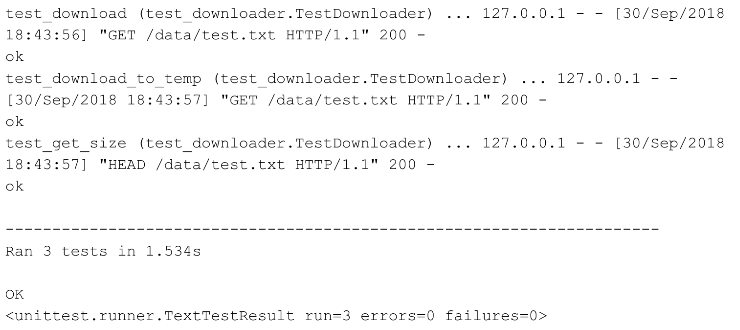
\includegraphics[scale=0.5]{../imgs/Figure1.png}
\caption{A run of an included test file, test\textunderscore downloader.py.}
\label{Figure1}
\end{figure}
\subsection{Brief Team Evaluation}
Overall the project is very organized with some help on building the project provided and only a little lacking information on testing what they have made. The developers were prepared for testing everything they needed to have tested, but only for themselves. It would have been more helpful for others looking in if there was a file that would automate the testing or at least more information on how to set up each individual test. We look forward to creating our own tests and exploring in more detail this project.

\end{document}